\documentclass[11pt,a4paper]{article}

\usepackage[utf8]{inputenc}
\inputencoding{utf8}
\usepackage{graphicx}
\usepackage{caption}
\usepackage{subcaption}
\usepackage[brazil]{babel}
\usepackage{amsmath,amssymb}
\usepackage{float}
\usepackage{url}

\title{Avaliação do HTML5 canvas em dispositivos móveis}
\author{
        André Guedes Linhares\\
        Centro de Informática - CIn UFPE\\
            \and
        Thiago de Barros Lacerda\\
        Centro de Informática - CIn UFPE\\
}
\date{\today}

\begin{document}
\maketitle

\section{Introdução}

A nova especificação do HTML, o HTML5, inclui um novo elemento visando facilitar o desenvolvimento de aplicações
dinâmicas e fluídas para internet, elemento esse chamado de canvas. De acordo com a especificação do HTML5
\cite{html5spec}, o canvas é um bitmap dependente de resolução que pode ser utilizado para renderizar gráficos,
elementos gráficos de jogos, arte e qualquer outro tipo de imagem em tempo real.

O canvas permite ao usuário, adicionar interatividade à paginas web, deixando o usuário controlar gráficos, imagens e
fotos dinamicamente utilizando linguagem de script.

Por causa do canvas, o HTML5 vem sendo vastamente utilizado para desenvolver aplicativos e jogos, não só web, mas também
para dispositivos móveis. Isso se dá ao fato de browsers e engines de renderização HTML darem suporte ao canvas
nativamente, fazendo assim que o HTML5 se torne uma ferramenta muito poderosa para desenvolver aplicativos e jogos que
rodem em diferentes plataformas, usando o mesmo código. Outros pontos importantes que vêm aumentando a utilização do
canvas:
\begin{enumerate}
    \item Facilidade de transformar uma página web estática em uma aplicação web dinâmica, para ser usada em smartphones
    e tablets.
    \item Forte candidato a substituir o Flash, pela sua facilidade de interagir com elementos da página, pois ele não
    deixa de ser um elemento HTML.
    \item Suportado nativamente nos browsers, o que remove a necessidade de plugins externos.
\end{enumerate}


\section{Objetivos}

Este trabalho visa fazer uma avaliação do canvas nos browsers mais utilizados em dispositivos móveis, o Chrome e o
Safari. Para isso utilizamos dois tablets bastante utilizados, o Nexus 7 e o iPad 3.

Nossos experimentos procuraram avaliar em geral qual seria o melhor browser, rodando em qual sistema operacional e
em qual dispositivo, para rodar uma aplicação HTML5 utilizando o canvas.

\section{Metodologia}
Para fazer a avaliação do canvas HTML5 utilizamos o teste em \cite{benchmark}, que consiste em avaliar operações que são
comuns em jogos e aplicações web utilizando o canvas, tais como: desenho de linhas horizontais e verticais, desenho de
múltiplos retângulos preenchidos, desenho de arcos, desenho de figuras, rotação de objetos, entre outros. O teste tenta
fazer o máximo de operações em um segundo, onde cada operação tem um peso relativo a sua importância e utilização numa
aplicação. No fim uma nota é atribuída ao browser que está rodando o teste, nota esta dependente de quantas operações o
browser conseguiu executar.

Como citado na seção anterior, utilizamos o Nexus 7 (rodando o sistema operaional Android) e o iPad 3 (rodando o sistema
operacional iOS). Para os testes no Nexus 7 utilizamos o Chrome \cite{chrome} (browser mais utilizado nessa plataforma)
rodando em duas versões diferentes de Android \cite{android}, a 4.4 (KitKat) e a 4.3 (Jelly Bean). No iPad 3, rodamos os
testes no browser nativo do sistema, o Safari \cite{safari}, utilizando o iOS 7 \cite{ios7}.

Para cada par [Sistema Operacional, browser], rodamos duas baterias do teste \cite{benchmark}, uma com 500 amostras e
outra com 200. Com esses dados em mãos fizemos algumas análises estatísticas tendo como objetivo comparar a performance
do canvas de cada par.

\section{Análise Descritiva}\label{analise descritiva}

Primeiro foi realizado uma análise visando extrair alguns estimadores estatísticos para as amostras, como: média,
mediana, desvio padrão, amplitude, curtose e assimetria. A tabela~\ref{descritiva} mostra os resultados obtidos.

\begin{table}[H]
    \centering
    \caption{Análise descritiva - 500 amostras}
    \label{descritiva}
    \begin{tabular}{| l | l | l | l |}
    \hline
     & Android 4.3 & Android 4.4 & iPad 3 \\ \hline
    Média & 0.923 & 1.598 & 0.918 \\ \hline
    Mediana & 0.918 & 1.6 & 0.919 \\ \hline
    Desvio padrão & 0.026 & 0.019 & 0.007 \\ \hline
    Amplitude & 0.11 & 0.14 & 0.087 \\ \hline
    Curtose & -1.4 & 0.238 & 24.405 \\ \hline
    Assimetria & 0.121 & -0.119 & -2.758 \\ \hline
    \end{tabular}
\end{table}

Além da análise feita acima, para cada par analisado plotamos seus histogramas de densidade e frequência, a ECDF e realizamos um teste de hipótese
entre pares para verificar se suas performances são iguais ou não.

\subsection{ECDFs}\label{ecdfs}

É possível notar na figura~\ref{ipadecdfs} que o desempenho do Safari, rodando no iOS 7 no iPad 3, na grande maioria das
vezes alcança uma nota entre 0.92 e 0.94 e que seu comportamento continua similar mesmo aumentando o número de amostras
analisadas.

\begin{figure}[H]
    \caption{ECDFs - iPad 3 Safari}
    \label{ipadecdfs}
    \begin{subfigure}{.5\textwidth}
        \caption{500 amostras}
        \centering
        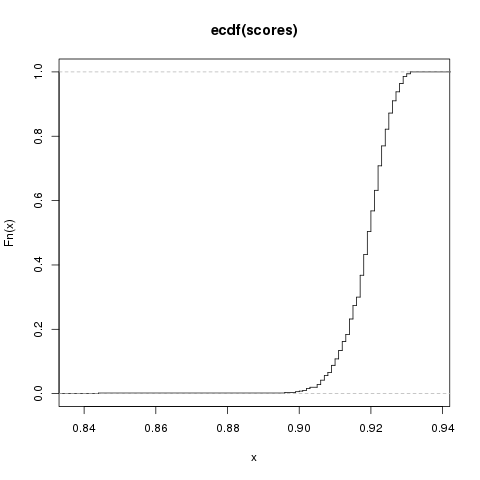
\includegraphics[width=\textwidth]{images/ecdf-ipad-3-ios7-safari-500-amostras-20131119}
        \label{safari500}
    \end{subfigure}
    \begin{subfigure}{.5\textwidth}
        \caption{200 amostras}
        \centering
        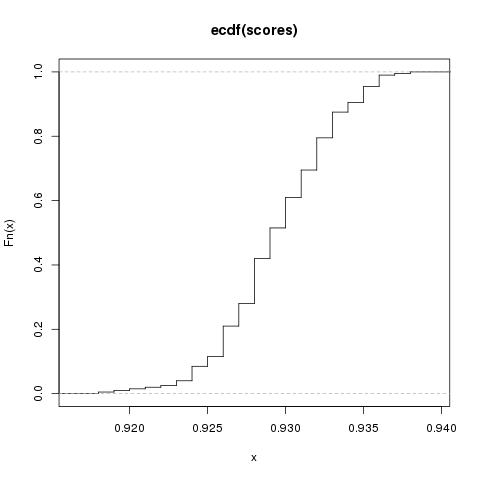
\includegraphics[width=\textwidth]{images/ecdf-ipad-3-ios7-safari-200-amostras-20131126}
        \label{safari200}
    \end{subfigure}
\end{figure}

Ao comparar o desempenho do Safari com o do Chrome rodando no Android 4.3, podemos perceber, pela
figura~\ref{nexus43ecdfs} que o Chrome se sai melhor do que o Safari, tendo suas notas variando na maioria entre 0.93 e
0.98.

\begin{figure}[H]
    \caption{ECDFs - Nexus 7, Android 4.3 Chrome}
    \label{nexus43ecdfs}
    \begin{subfigure}{.5\textwidth}
        \caption{500 amostras}
        \centering
        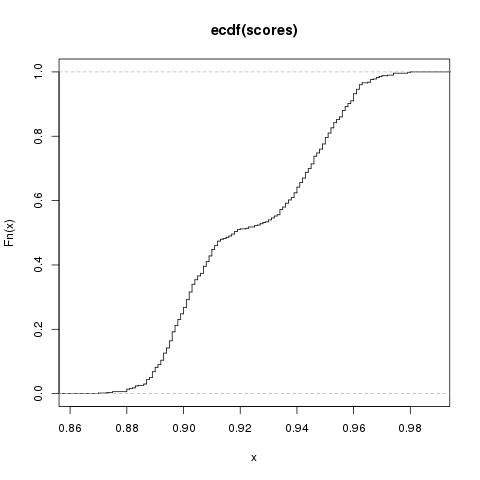
\includegraphics[width=\textwidth]{images/ecdf-n7-a43-chrome-500-amostras-20131119}
        \label{nexus43500}
    \end{subfigure}
    \begin{subfigure}{.5\textwidth}
        \caption{200 amostras}
        \centering
        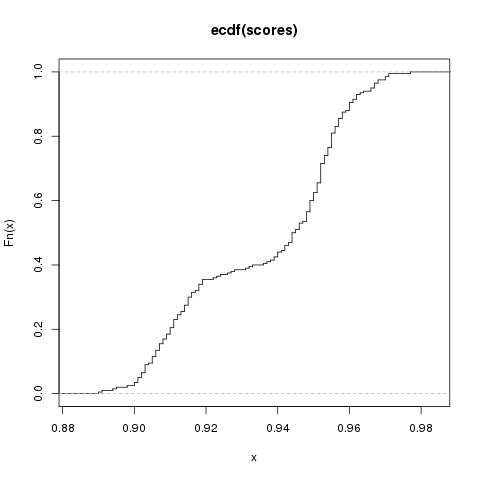
\includegraphics[width=\textwidth]{images/ecdf-n7-a43-chrome-200-amostras-20131120}
        \label{nexus43200}
    \end{subfigure}
\end{figure}

Na figura~\ref{nexus44ecdfs} nota-se que seu desempenho é superior a todos os outros analisados previamente, tendo suas
notas variando, na maioria das vezes, entre 1.5 e 1.6.

\begin{figure}[H]
    \caption{ECDFs - Nexus 7, Android 4.4 Chrome}
    \label{nexus44ecdfs}
    \begin{subfigure}{.5\textwidth}
        \caption{500 amostras}
        \centering
        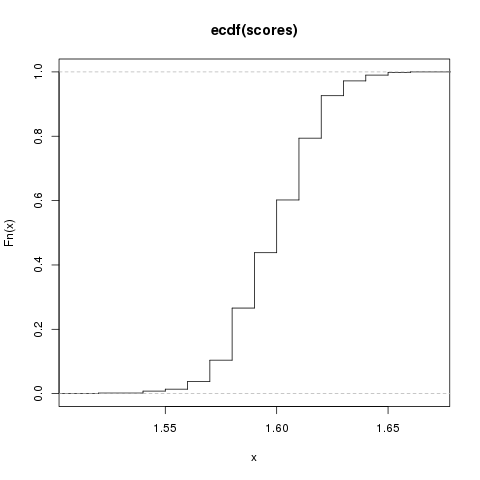
\includegraphics[width=\textwidth]{images/ecdf-n7-a44-chrome-500-amostras-20131119}
        \label{nexus44500}
    \end{subfigure}
    \begin{subfigure}{.5\textwidth}
        \caption{200 amostras}
        \centering
        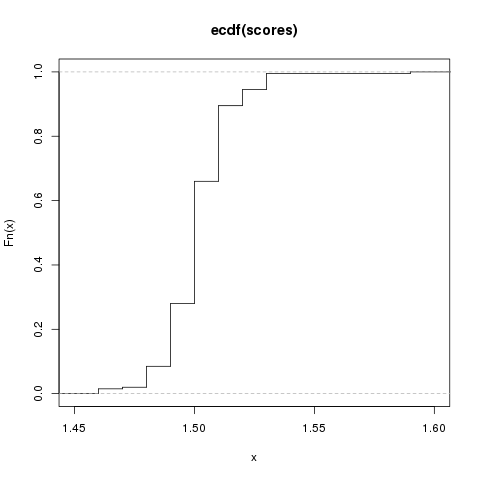
\includegraphics[width=\textwidth]{images/ecdf-n7-a44-chrome-200-amostras-20131120}
        \label{nexus44200}
    \end{subfigure}
\end{figure}


\subsection{Histogramas}\label{histogramas}

Abaixo apresentamos os histogramas dos browsers analisados, podemos observar que eles só confirmam as afirmações feitas
na seção anterior, onde o Chrome rodando no Android 4.4 supera todos os outros. Da análise dos histogramas foi possível
concluir também que nenhuma das amostras conseguiram ser modeladas para uma normal, com o intuito de deixar isso claro
foi plotado também a curva normal que mais se aproximaria do histograma.

\begin{figure}[H]
    \caption{Histogramas - iPad 3 Safari}
    \label{safarihistogramas}
    \begin{subfigure}{.5\textwidth}
        \caption{500 amostras}
        \centering
        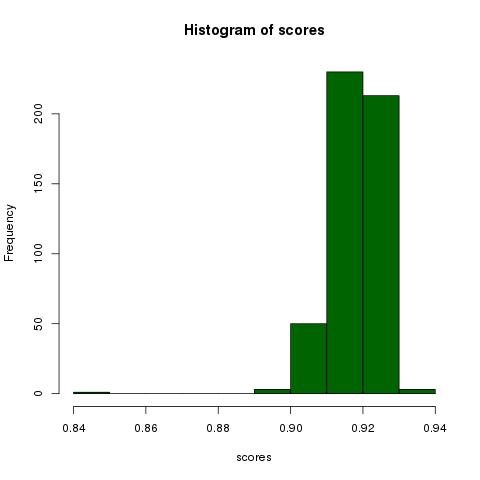
\includegraphics[width=\textwidth]{images/hist-freq-ipad-3-ios7-safari-500-amostras-20131119}
        \label{safarihistograma500}
    \end{subfigure}
    \begin{subfigure}{.5\textwidth}
        \caption{200 amostras}
        \centering
        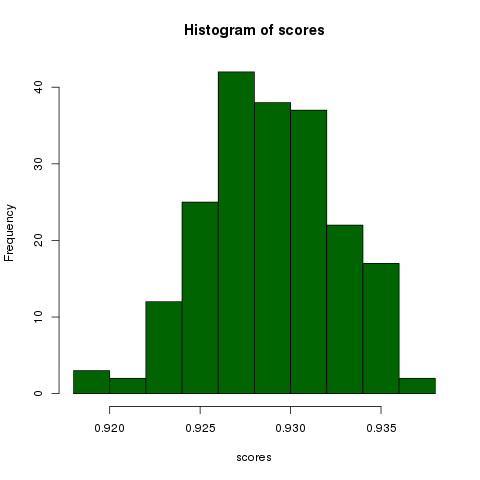
\includegraphics[width=\textwidth]{images/hist-freq-ipad-3-ios7-safari-200-amostras-20131126}
        \label{safarihistograma200}
    \end{subfigure}
\end{figure}

Na figura~\ref{nexus43histogramas}, onde apresentamos os histogramas para o Chrome rodand no Android 4.3, foi possível
observer um comportamento bimodal, onde temos dois picos de notas, bem diferente das outras amostras.

\begin{figure}[H]
    \caption{Histogramas - Nexus 7, Android 4.3 Chrome}
    \label{nexus43histogramas}
    \begin{subfigure}{.5\textwidth}
        \caption{500 amostras}
        \centering
        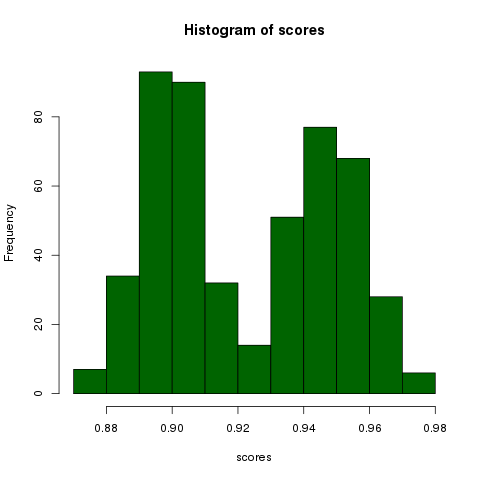
\includegraphics[width=\textwidth]{images/hist-freq-n7-a43-chrome-500-amostras-20131119}
        \label{nexus43histograma500}
    \end{subfigure}
    \begin{subfigure}{.5\textwidth}
        \caption{200 amostras}
        \centering
        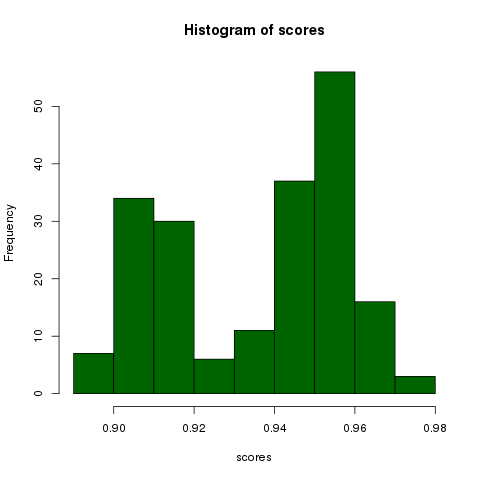
\includegraphics[width=\textwidth]{images/hist-freq-n7-a43-chrome-200-amostras-20131120}
        \label{nexus43histograma200}
    \end{subfigure}
\end{figure}

\begin{figure}[H]
    \caption{Histogramas - Nexus 7, Android 4.4 Chrome}
    \label{nexus44histogramas}
    \begin{subfigure}{.5\textwidth}
        \caption{500 amostras}
        \centering
        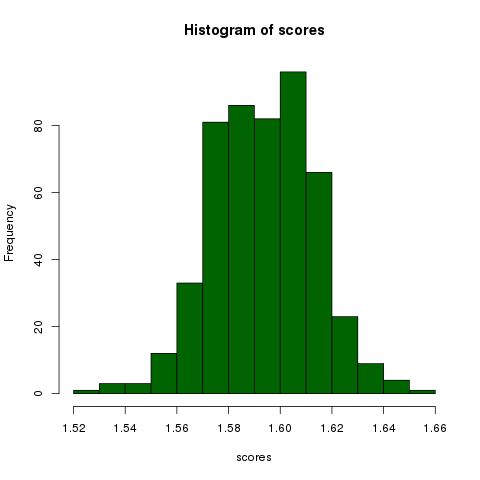
\includegraphics[width=\textwidth]{images/hist-freq-n7-a44-chrome-500-amostras-20131119}
        \label{nexus44histograma500}
    \end{subfigure}
    \begin{subfigure}{.5\textwidth}
        \caption{200 amostras}
        \centering
        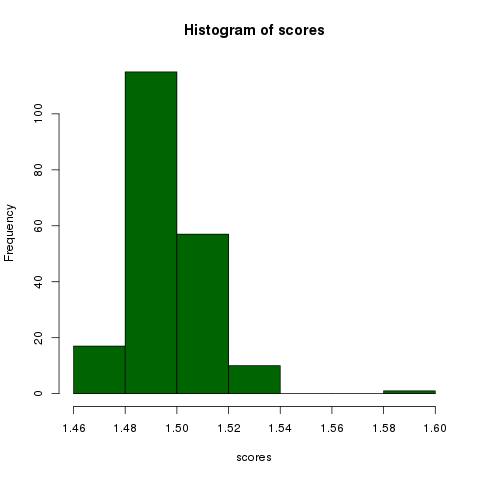
\includegraphics[width=\textwidth]{images/hist-freq-n7-a44-chrome-200-amostras-20131120}
        \label{nexus44histograma200}
    \end{subfigure}
\end{figure}

Abaixo mostramos os histogramas de densidade para os mesmos dispositivos e browsers analisados acima. Foi plotada também
a curva da distribuição normal que mais se aproximaria da distribuição da amostra, onde é possível observar que as
amostras não seguem uma distribuição normal. Apresentamos apenas os dados para 500 amostras, pois as de 200 apresentam o
mesmo padrão.

\begin{figure}[H]
    \caption{Histograma Densidade, 500 amostras - Nexus 7, Android 4.3 Chrome}
    \label{nexus43histogramadensidade}
    \centering
    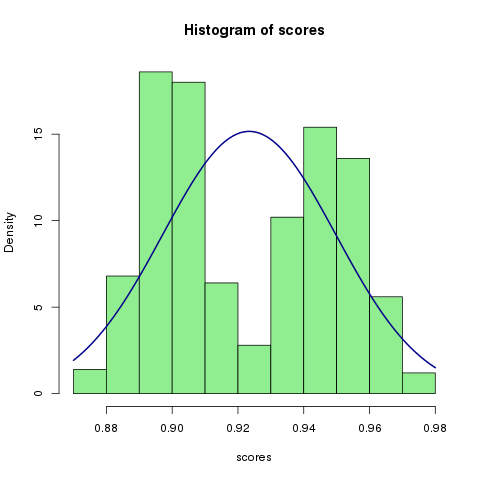
\includegraphics[width=\textwidth]{images/hist-density-n7-a43-chrome-500-amostras-20131119}
\end{figure}

\begin{figure}[H]
    \caption{Histograma Densidade, 500 amostras - Nexus 7, Android 4.4 Chrome}
    \label{nexus44histogramadensidade}
    \centering
    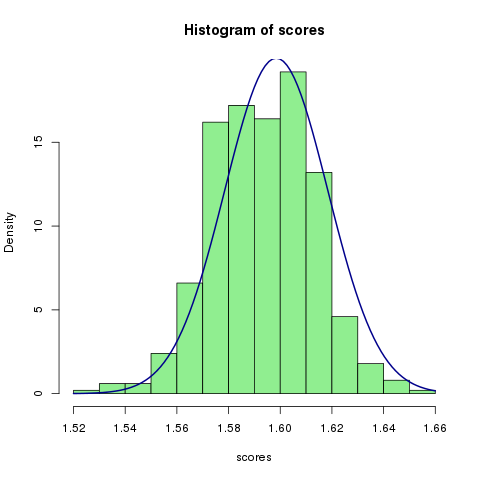
\includegraphics[width=\textwidth]{images/hist-density-n7-a44-chrome-500-amostras-20131119}
\end{figure}

\begin{figure}[H]
    \caption{Histograma Densidade, 500 amostras - iPad 3}
    \label{ipadhistogramadensidade}
    \centering
    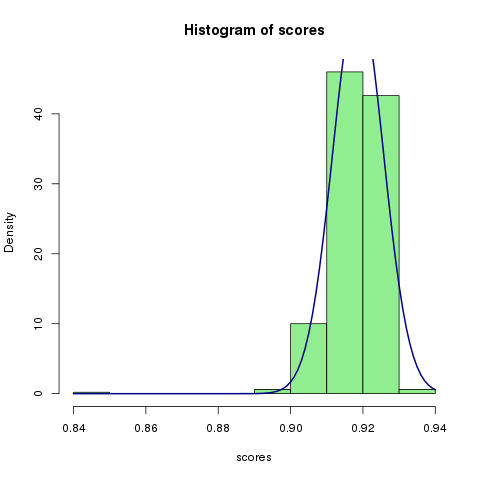
\includegraphics[width=\textwidth]{images/hist-density-ipad-3-ios7-safari-500-amostras-20131119}
\end{figure}

\section{Inferência}\label{inferencia}
Aqui vamos tentar inferir qual o dispositivo tem o melhor desempenho no canvas do HTML5, para isso fizemos testes de
hipóteses entre os dispositivos analisados.

Para escolher o teste correto, primeiro realizamos o Teste de Aderência KS, para saber se nossas amostras podem ser
aproximadas a uma distribuição normal. Para todas as inferências utilizamos o \(alpha\) igual a 0.05. Abaixo mostramos a
tabela dos P-values obtidos nos testes de aderência para cada dispositivo, com 500 amostras.

\begin{table}[H]
    \centering
    \caption{Teste KS - 500 amostras}
    \begin{tabular}{| l | l | l | l |}
    \hline
     & Android 4.3 & Android 4.4 & iPad 3 \\ \hline
    P-value & 0.000035 & 0.003 & 0.011 \\ \hline
    \end{tabular}
\end{table}

Pela tabela acima, podemos ver que nossas amostras não podem ser aproximados para uma distribuição normal. Esse
comportamento também se repete para 200 amostras.

\subsection{Teste de hipótese}\label{testedehipotese}

Por último, um teste de hipótese foi feito comparando cada dispositivo analisado. Para cada par, criamos as seguintes
hipóteses:

\begin{align*}
        H_0: \mu_0 = \mu_1 \\
        H_1: \mu_0 > \mu_1
\end{align*}

Onde a hipótese nula afirma que os dispositivos comparados tem um desempenho igual em média e a hipótese alternativa
diz que a média do primeiro dispositivo, \(\mu_0\), é maior que a do segundo dispositivo, \(\mu_1\).

Visto que os dados das nossas amostras não podem ser aproximados a uma normal, utilizamos teste não paramétrico de
Wilcoxon com o \(\alpha\) de 0.05, para poder testar as hipóteses propostas. A tabela~\ref{tabela1} resume os
resultados dos testes.

\begin{table}[H]
    \footnotesize
    \caption{Teste de Hipótese Wilcoxon - 500 amostras}
    \begin{tabular}{| l | l | l | l |}
    \hline
     & iPad 3 x Android 4.3 & iPad 3 x Android 4.4 & Android 4.3 x Android 4.4 \\ \hline
    \( H_0: \mu_0 = \mu_1 \) & não rejeita & rejeita & rejeita \\ \hline
    \( H_0: \mu_0 > \mu_1 \) & rejeita & não rejeita & não rejeita \\ \hline
    \end{tabular}
    \label{tabela1}
\end{table}

\section{Conclusão}\label{conclusao}

Com os experimentos apresentados, podemos concluir que, para uma aplicação web utilizando o canvas, o Chrome rodando no
Android 4.4 foi o que apresentou o melhor desempenho e o iPad 3 tem desempenho estatisticamente semelhante ao Android
4.3.

\bibliographystyle{abbrv}
\bibliography{stat}

\end{document}
This is never printed
